%-----------------------Homework------------------------------------
%-------------------Arman Shokrollahi---------------------------------
%---------------------Coding Theory-------------------------------

\documentclass[a4 paper]{article}
% Set target color model to RGB
\usepackage[inner=1.5cm,outer=1.5cm,top=2.5cm,bottom=2.5cm]{geometry}
\usepackage{setspace}
\usepackage[rgb]{xcolor}
\usepackage{pythonhighlight}
\usepackage{caption}
\usepackage{subcaption}
\usepackage{pdfpages}
\usepackage{verbatim}
\usepackage{amsgen,amsmath,amstext,amsbsy,amsopn,tikz,amssymb,tkz-linknodes}
\usepackage{fancyhdr}
\usepackage[colorlinks=true, urlcolor=blue,  linkcolor=blue, citecolor=blue]{hyperref}
\usepackage[colorinlistoftodos]{todonotes}
\usepackage{rotating}
%\usetikzlibrary{through,backgrounds}
\hypersetup{%
pdfauthor={Arman Shokrollahi},%
pdftitle={Homework},%
pdfkeywords={Tikz,latex,bootstrap,uncertaintes},%
pdfcreator={PDFLaTeX},%
pdfproducer={PDFLaTeX},%
}
%\usetikzlibrary{shadows}
\usepackage[francais]{babel}
\usepackage{booktabs}
\newcommand{\ra}[1]{\renewcommand{\arraystretch}{#1}}

      \newtheorem{thm}{Theorem}[section]
      \newtheorem{prop}[thm]{Proposition}
      \newtheorem{lem}[thm]{Lemma}
      \newtheorem{cor}[thm]{Corollary}
      \newtheorem{defn}[thm]{Definition}
      \newtheorem{rem}[thm]{Remark}
      \numberwithin{equation}{section}

\newcommand{\homework}[6]{
   \pagestyle{myheadings}
   \thispagestyle{plain}
   \newpage
   \setcounter{page}{1}
   \noindent
   \begin{center}
   \framebox{
      \vbox{\vspace{2mm}
    \hbox to 6.28in { {\bf JWST Project \hfill} }
       \vspace{6mm}
       \hbox to 6.28in { {\Large \hfill #1 (#2)  \hfill} }
       \vspace{6mm}
       \hbox to 6.28in { {\it Instructor: #3 \hfill Student: #5} }
       %\hbox to 6.28in { {\it TA: #4  \hfill #6}}
      \vspace{2mm}}
   }
   \end{center}
   \markboth{#5 -- #1}{#5 -- #1}
   \vspace*{4mm}
}

\newcommand{\bbF}{\mathbb{F}}
\newcommand{\bbX}{\mathbb{X}}
\newcommand{\bI}{\mathbf{I}}
\newcommand{\bX}{\mathbf{X}}
\newcommand{\bY}{\mathbf{Y}}
\newcommand{\bepsilon}{\boldsymbol{\epsilon}}
\newcommand{\balpha}{\boldsymbol{\alpha}}
\newcommand{\bbeta}{\boldsymbol{\beta}}
\newcommand{\0}{\mathbf{0}}

\begin{document}
\homework{Meeting Notes \#2}{due 02/22/23 }{McCleary}{}{Eddie Berman}{}
{\begin{tikzpicture}[outline/.style={draw=#1,thick,fill=#1!50}]
\node [outline=red] at (0,1) {\bf Agenda};
\end{tikzpicture}}
\begin{enumerate}
    \item New results from PSF
    \item Go through real data running because I'm a little confused
    \item Another Paper
    \item Ascent Award
    \item Steps toward understanding and making my own PIFF

\end{enumerate}

\noindent {\fbox{\it PSF Results}}\\ 
\section{First results from PSF}
\subsection{60mas Max Size Simulated Data}

\begin{python}
# How large should the postage stamp cutouts of the stars be?
    stamp_size: 30

model:
    # This model uses a grid of pixels to model the surface brightness distribution.
    type: PixelGrid
    scale: 0.025      # NIRCam ative pixel scale
    size: 60          # Model is 24 x 24 in these pixels
\end{python}\\
\begin{python}
    # Output 277
Iteration 1: Fitting 153 stars
             (27 stars are reserved)
Beginning solution of matrix size (21600, 21600)
Ill-conditioned matrix (rcond=4.89443e-20): result may not be accurate.
             Total chisq = 2719.75 / 137241 dof
Iteration 2: Fitting 153 stars
             (27 stars are reserved)
Beginning solution of matrix size (21600, 21600)
Ill-conditioned matrix (rcond=4.28319e-20): result may not be accurate.
             Total chisq = 1623.11 / 137241 dof
\end{python}
\begin{python}
    # Output 444
Iteration 1: Fitting 148 stars
             (25 stars are reserved)
Beginning solution of matrix size (21600, 21600)
Ill-conditioned matrix (rcond=1.43754e-19): result may not be accurate.
             Total chisq = 4094.30 / 132756 dof
Iteration 2: Fitting 148 stars
             (25 stars are reserved)
Beginning solution of matrix size (21600, 21600)
Ill-conditioned matrix (rcond=4.14087e-19): result may not be accurate.
\end{python}
\begin{figure}[!h]
  \begin{subfigure}{\linewidth}
  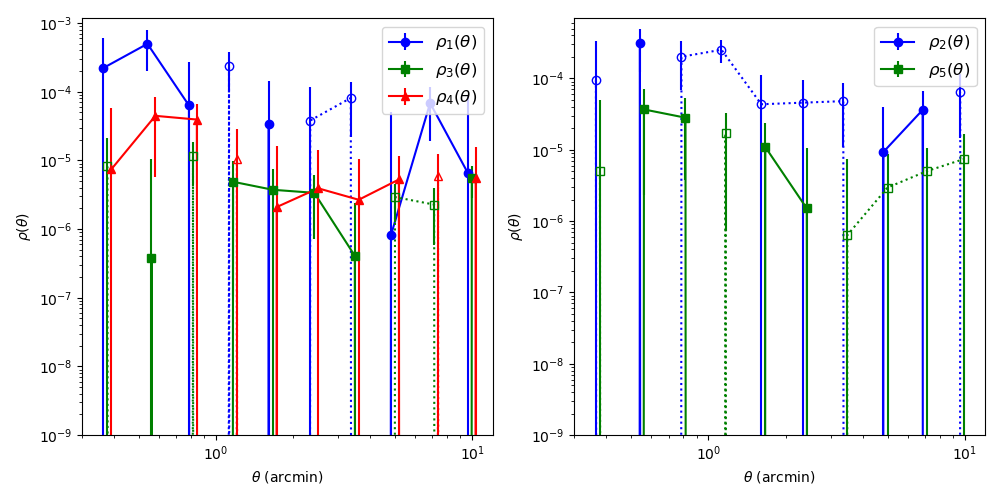
\includegraphics[width=.3\linewidth]{Simulated60mas277/piff_rho.png}\hfill
  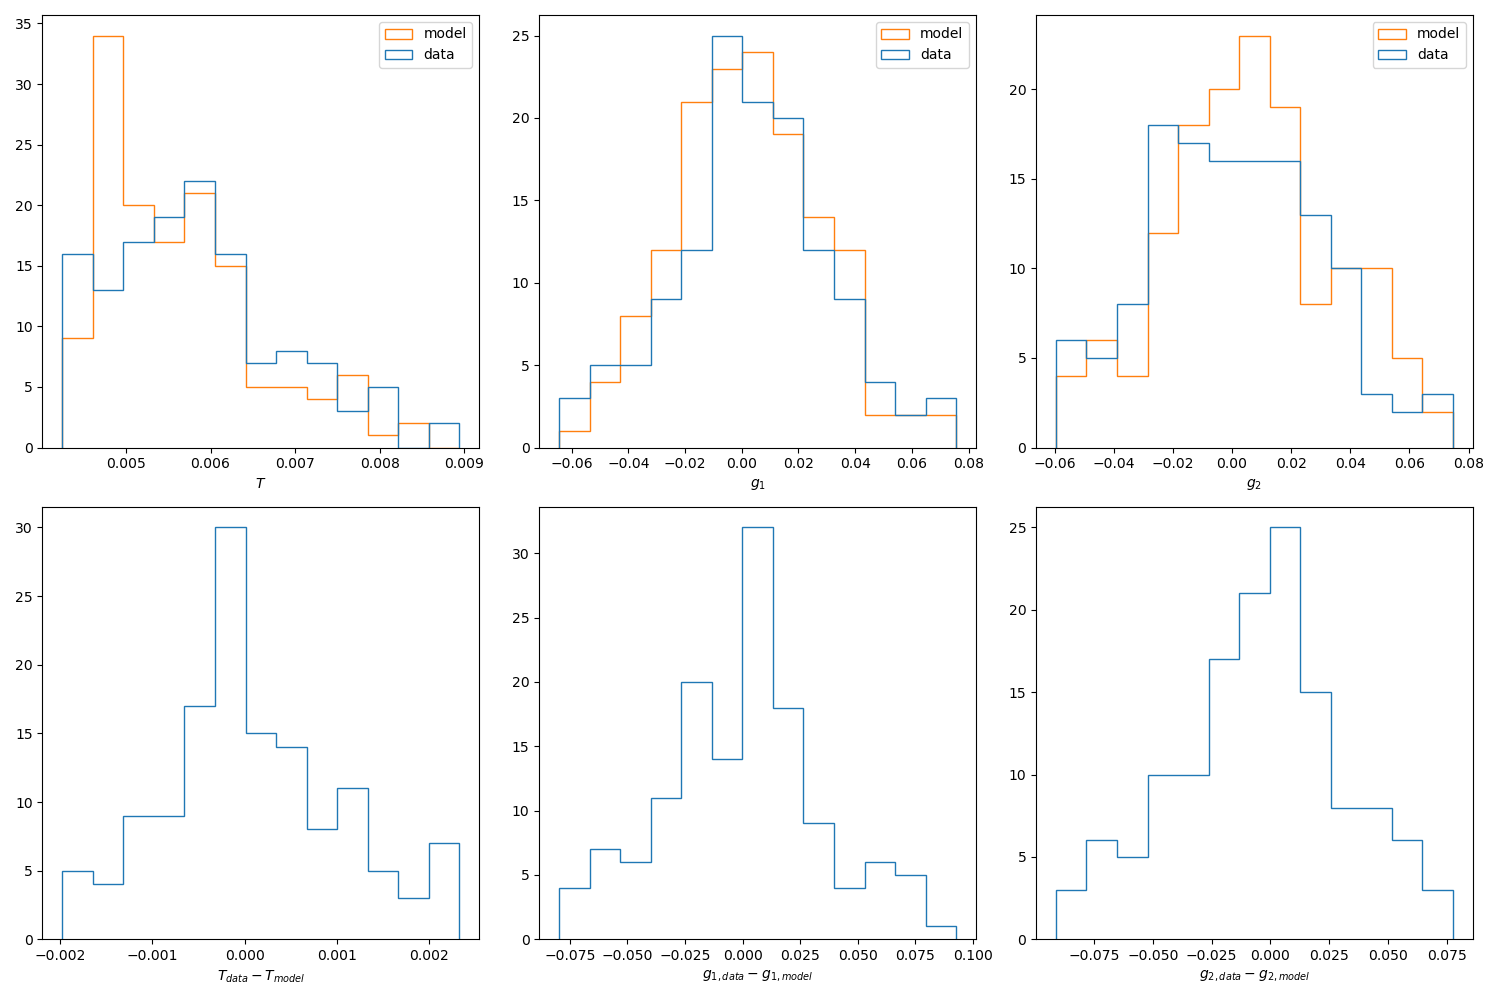
\includegraphics[width=.3\linewidth]{Simulated60mas277/piff_shapes.png}\hfill
  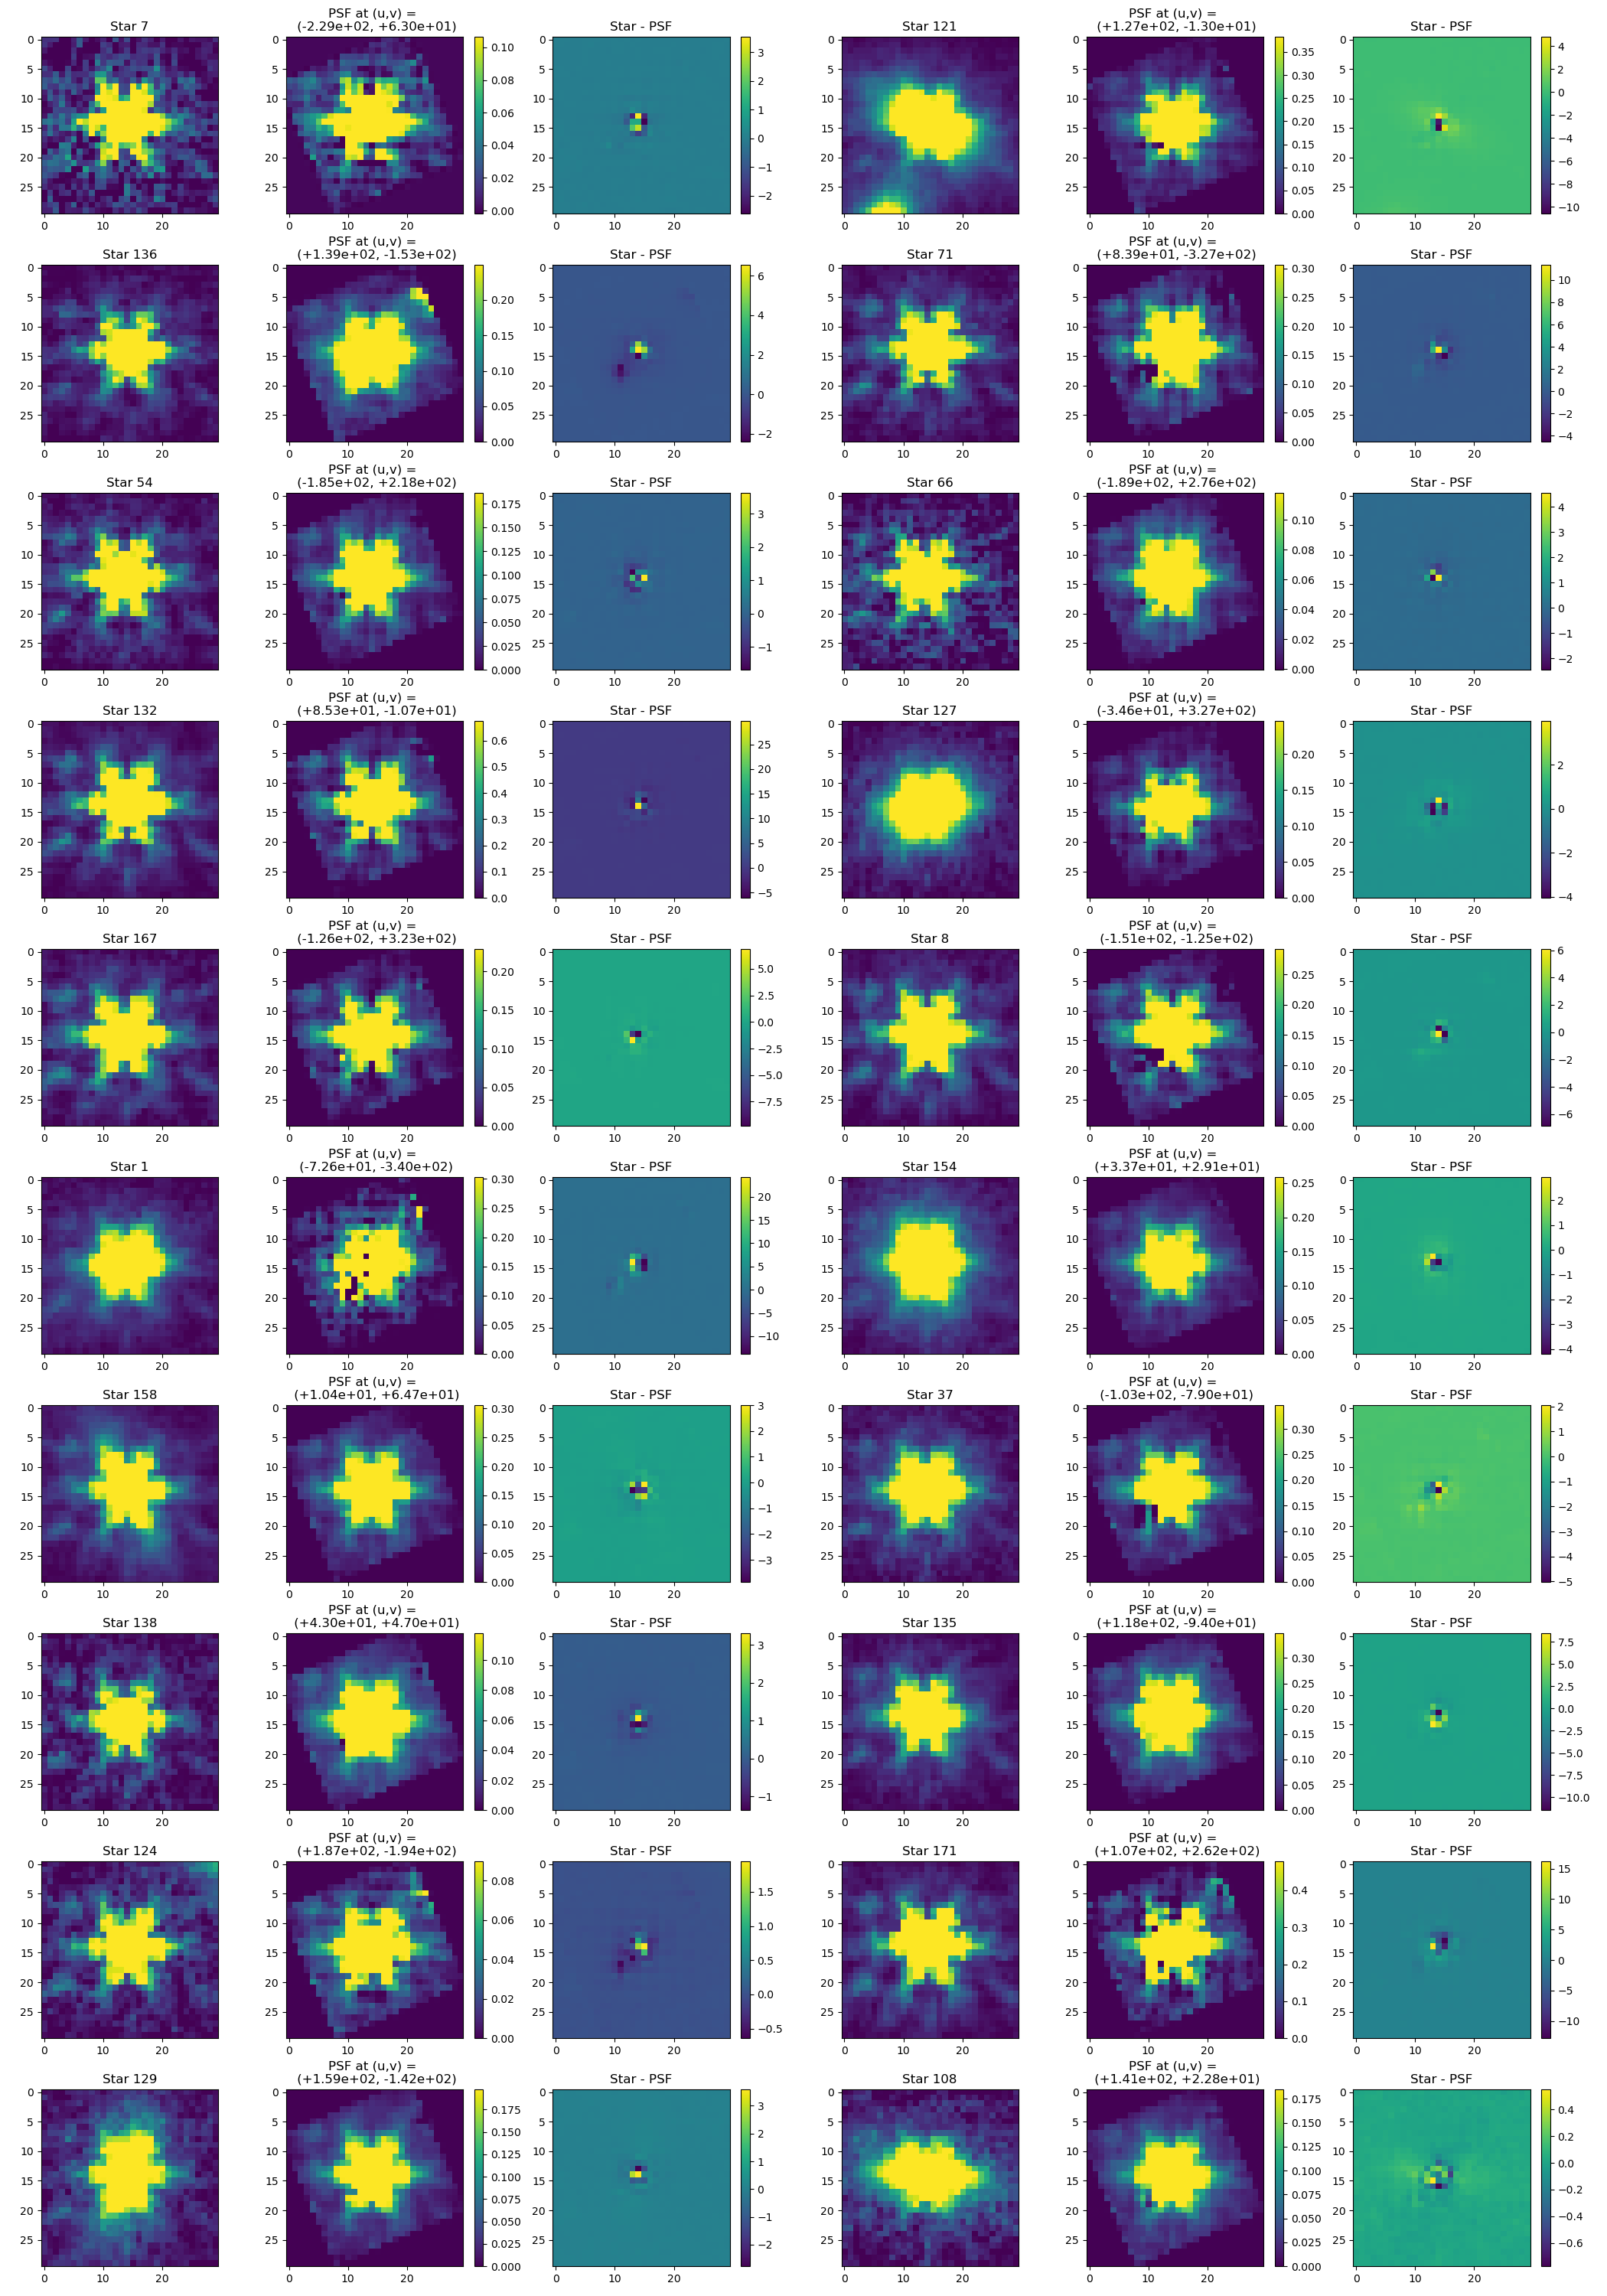
\includegraphics[width=.3\linewidth]{Simulated60mas277/piff_stars.png}
  \end{subfigure}\par\medskip
  \begin{subfigure}{\linewidth}
  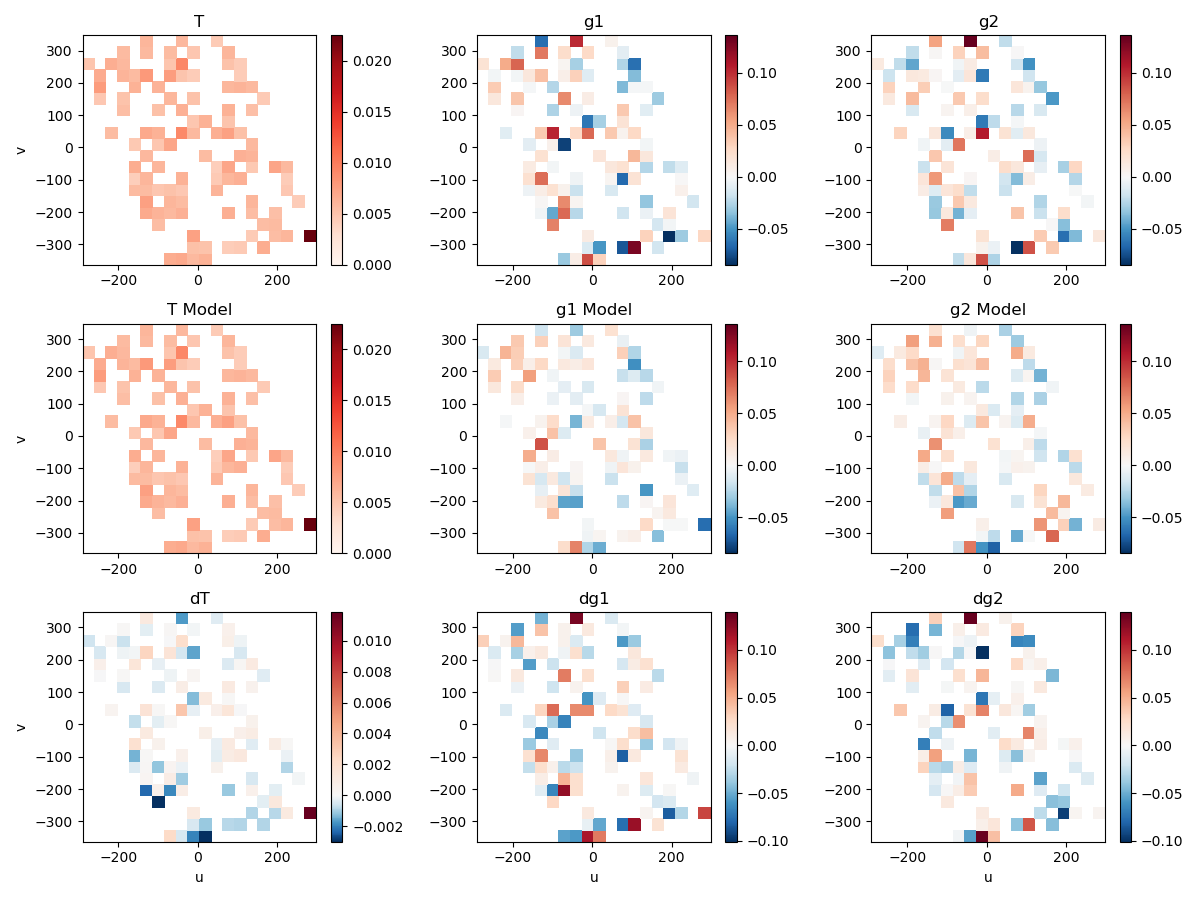
\includegraphics[width=.3\linewidth]{Simulated60mas277/piff_twod.png}\hfill
  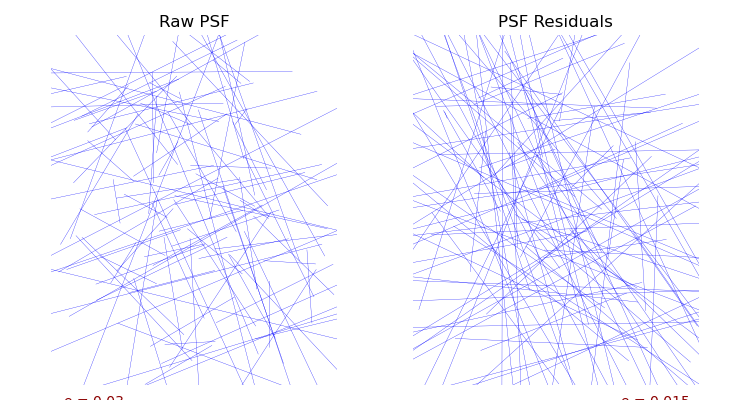
\includegraphics[width=.3\linewidth]{Simulated60mas277/piff_whisker.png}\hfill
  \caption{Simulated60mas277}
  \end{subfigure}\par\medskip


\end{figure}
Comment, things break down heavily! See rcond number\\
In the second case things broke down in a more pathological way

\begin{figure}[!h]
  \begin{subfigure}{\linewidth}
  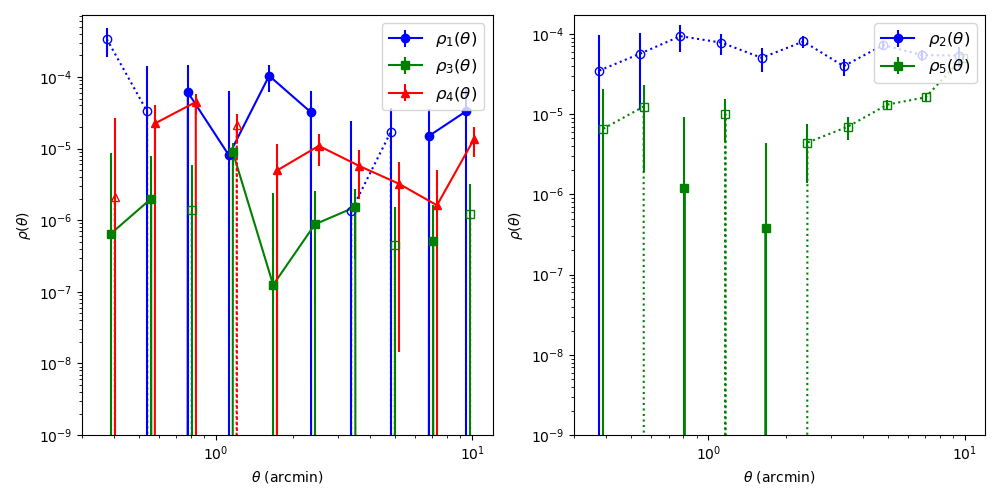
\includegraphics[width=.3\linewidth]{Simulated60mas444/piff_rho.png}\hfill
  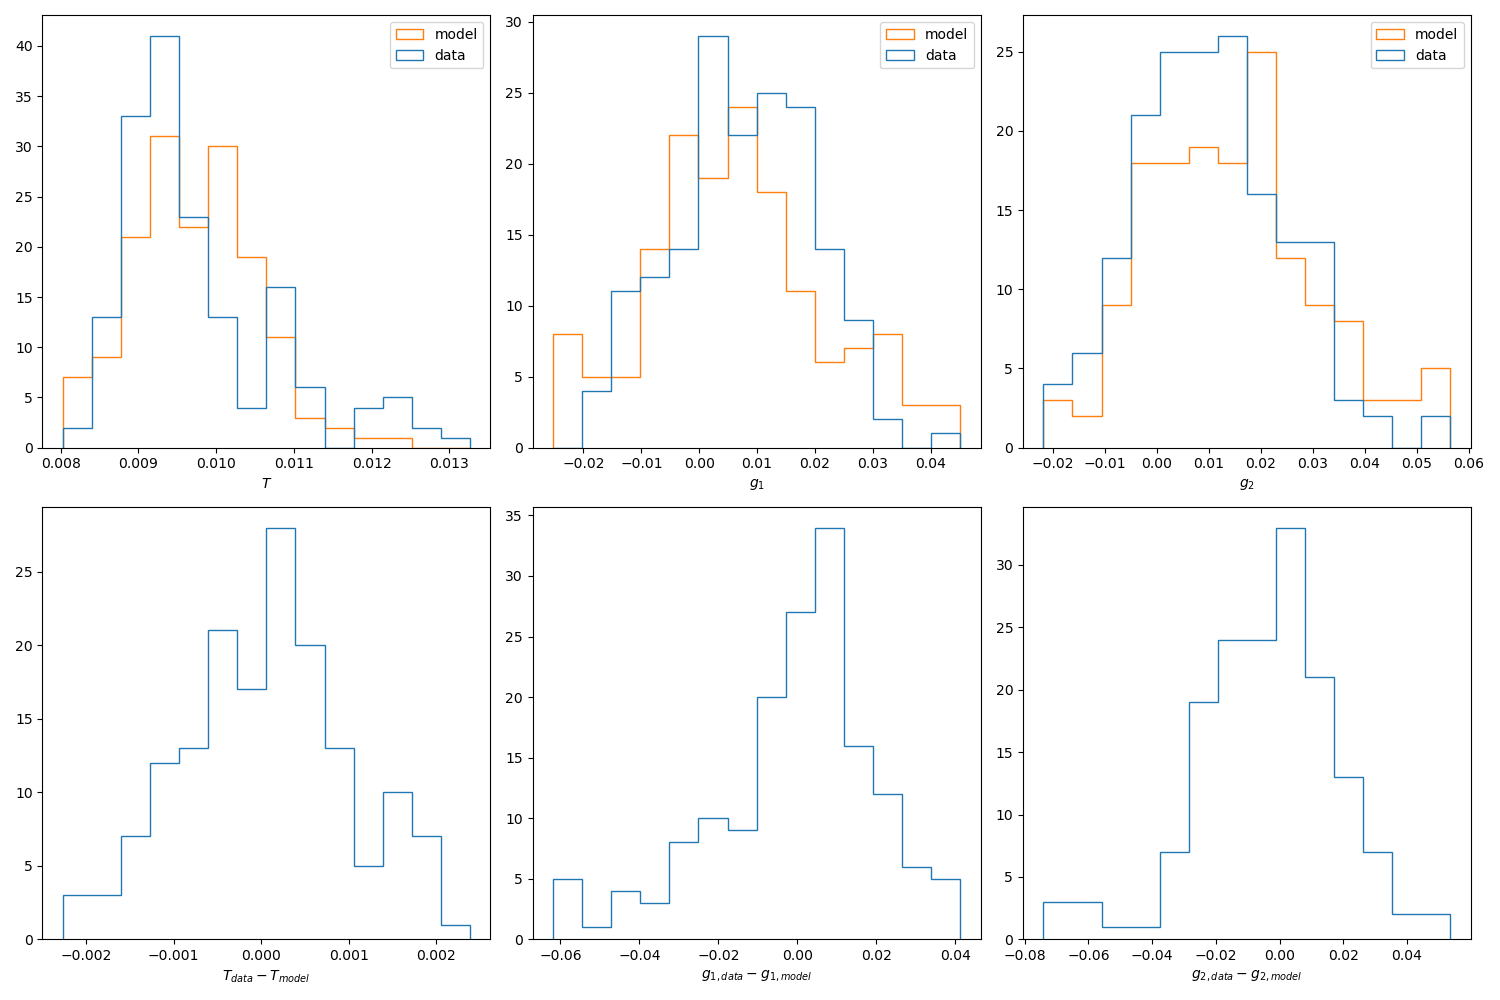
\includegraphics[width=.3\linewidth]{Simulated60mas444/piff_shapes.png}\hfill
  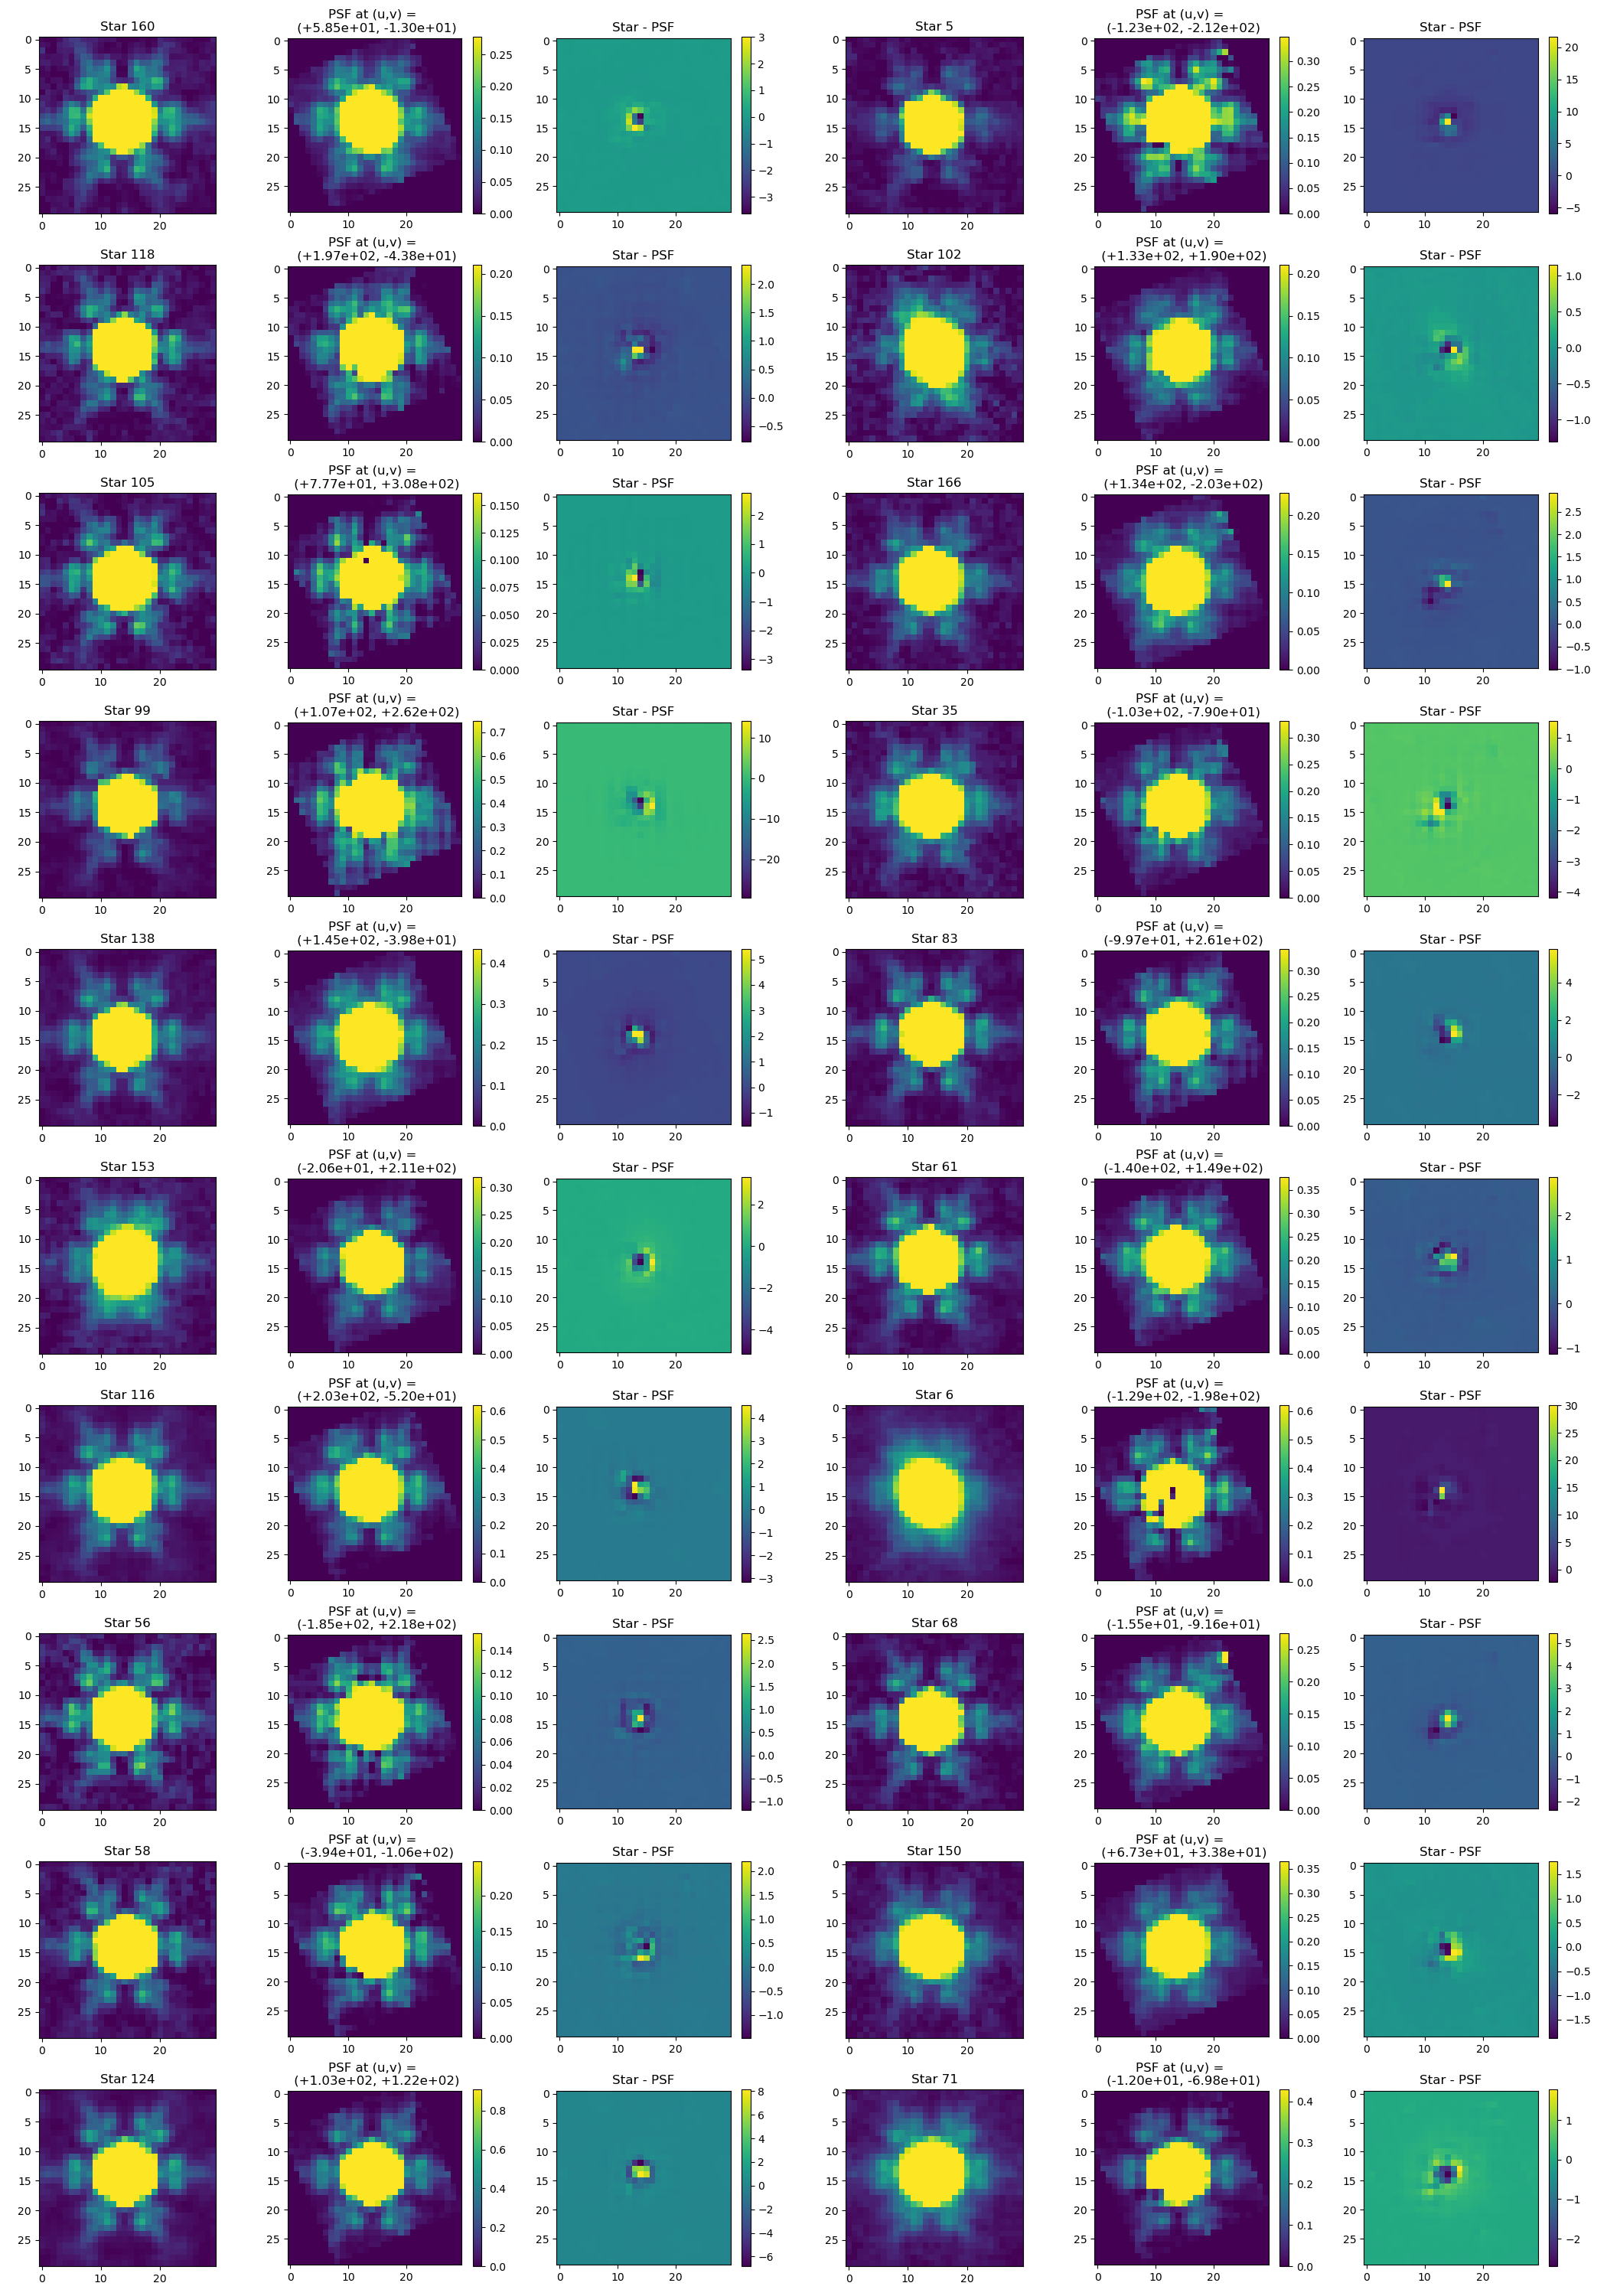
\includegraphics[width=.3\linewidth]{Simulated60mas444/piff_stars.png}
  \end{subfigure}\par\medskip
  \begin{subfigure}{\linewidth}
  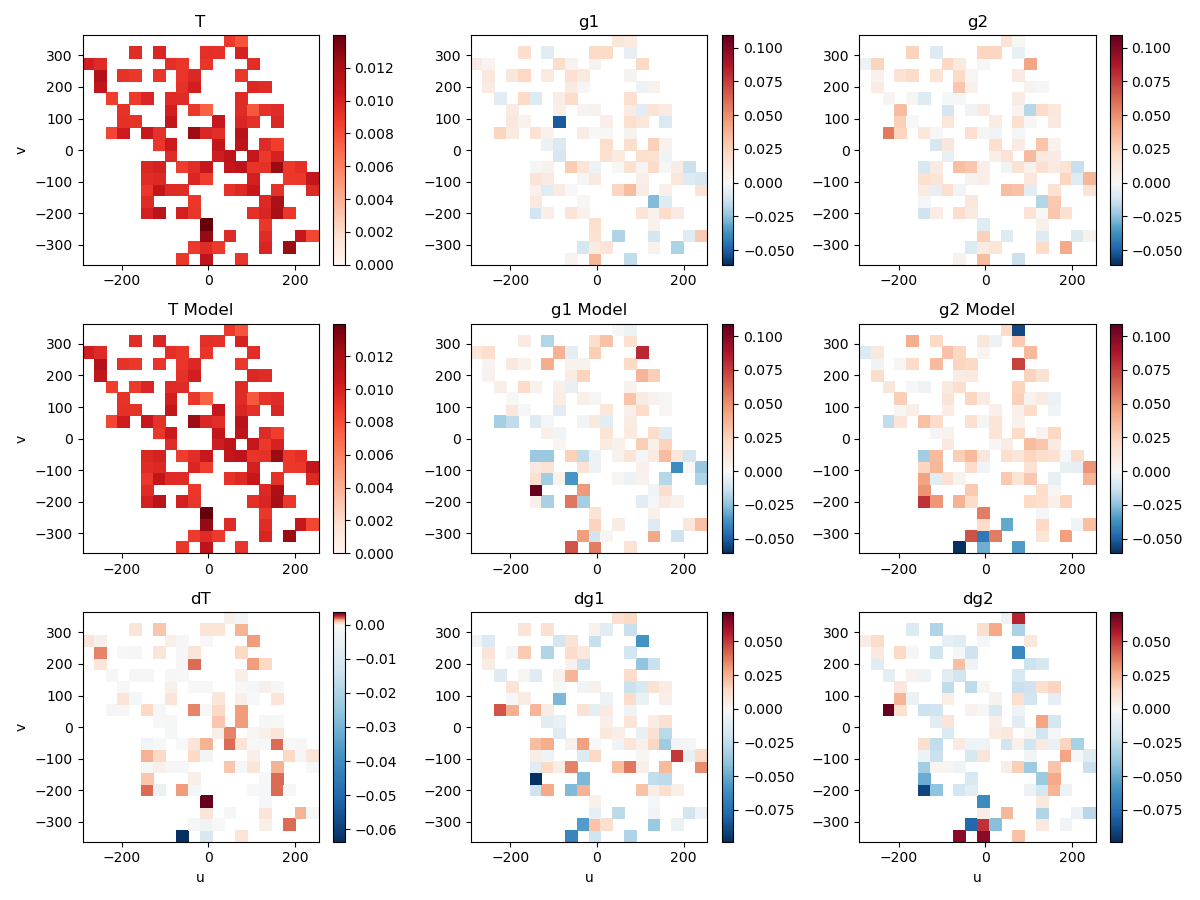
\includegraphics[width=.3\linewidth]{Simulated60mas444/piff_twod.png}\hfill
  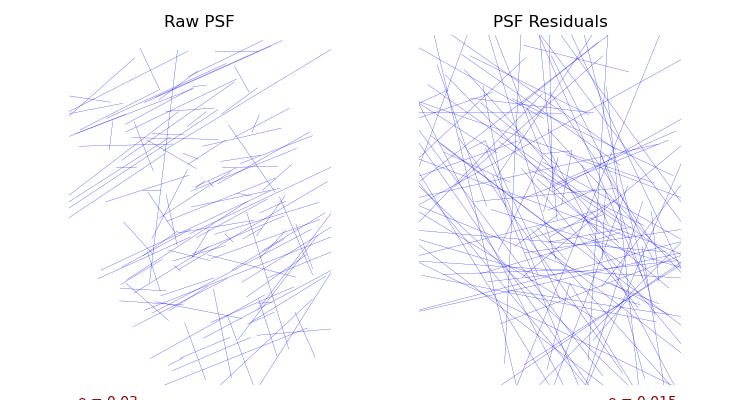
\includegraphics[width=.3\linewidth]{Simulated60mas444/piff_whisker.png}\hfill
  \caption{Simulated60mas444}
  \end{subfigure}\par\medskip


\end{figure}
\clearpage
\subsection{30mas Max Size Simulated Data}
\begin{python}
# How large should the postage stamp cutouts of the stars be?
    stamp_size: 30

model:
    # This model uses a grid of pixels to model the surface brightness distribution.
    type: PixelGrid
    scale: 0.025      # NIRCam ative pixel scale
    size: 35          # Model is 24 x 24 in these pixels
\end{python}\\
\begin{python}
    # Output 150
Iteration 1: Fitting 236 stars
             (41 stars are reserved)
Beginning solution of matrix size (9600, 9600)
Caught Matrix is singular.
Switching to svd solution

\end{python}\\
Then tried:
\begin{python}
# How large should the postage stamp cutouts of the stars be?
    stamp_size: 30

model:
    # This model uses a grid of pixels to model the surface brightness distribution.
    type: PixelGrid
    scale: 0.025      # NIRCam ative pixel scale
    size: 30          # Model is 24 x 24 in these pixels
\end{python}\\
\begin{figure}[!h]
  \begin{subfigure}{\linewidth}
  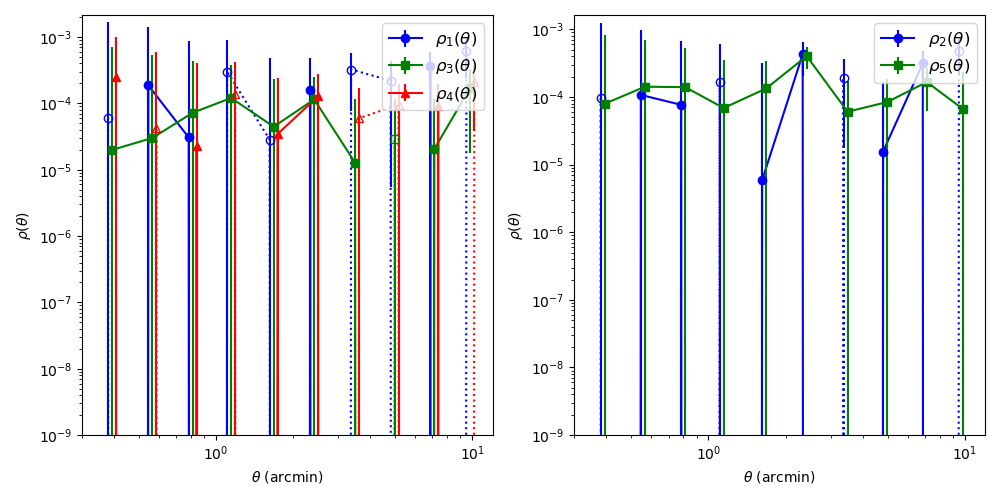
\includegraphics[width=.3\linewidth]{Simulated30mas115/piff_rho.png}\hfill
  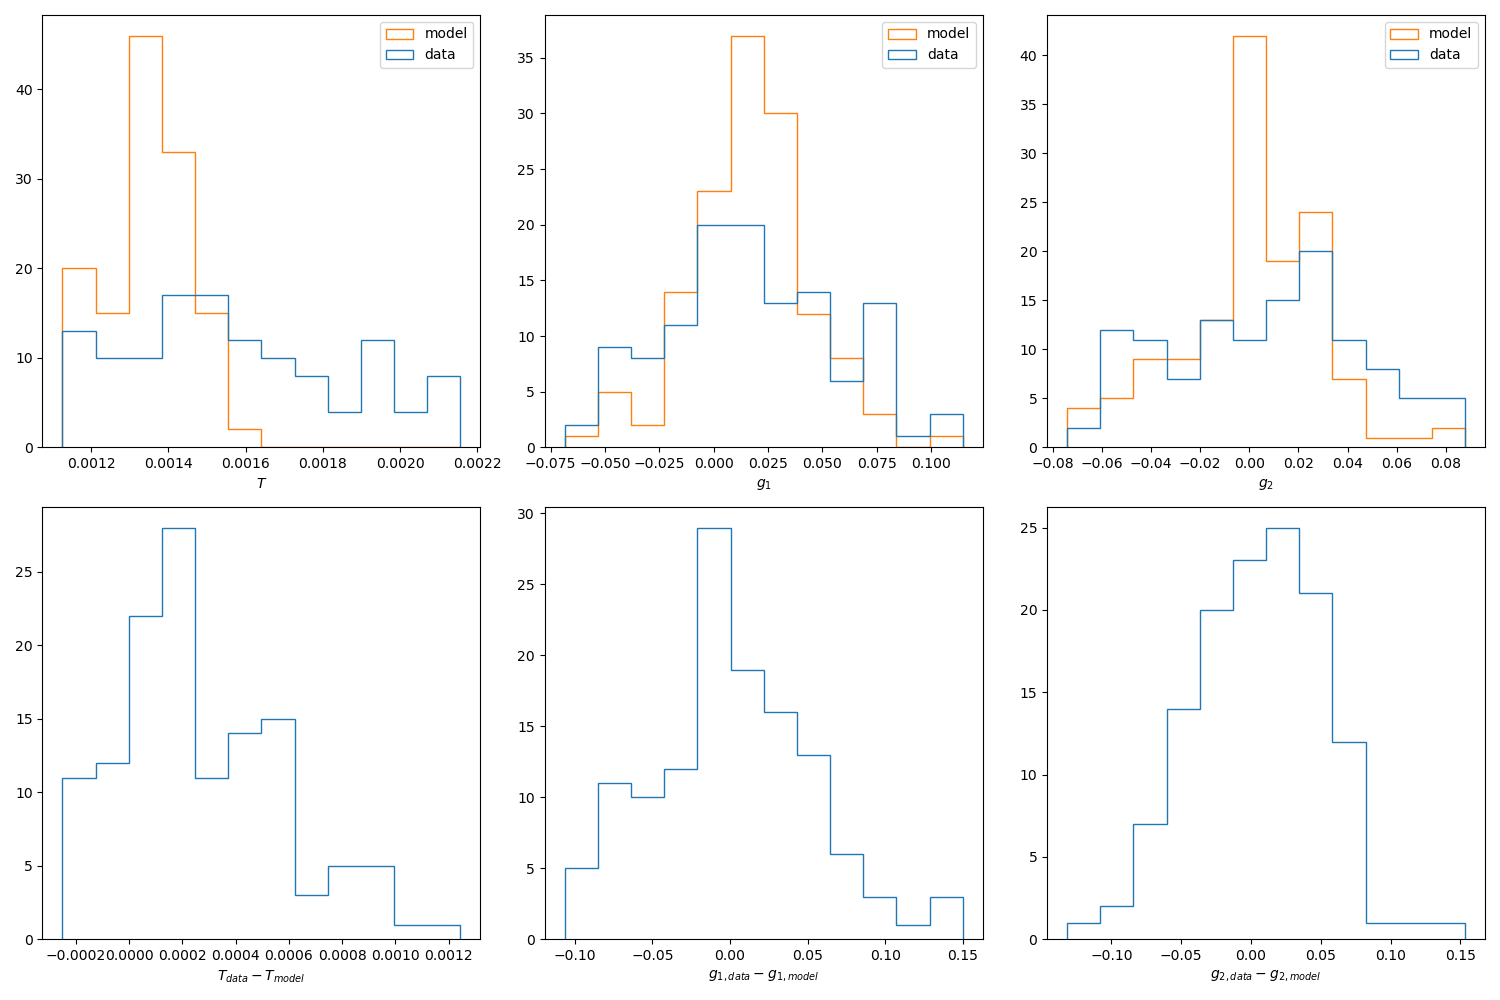
\includegraphics[width=.3\linewidth]{Simulated30mas115/piff_shapes.png}\hfill
  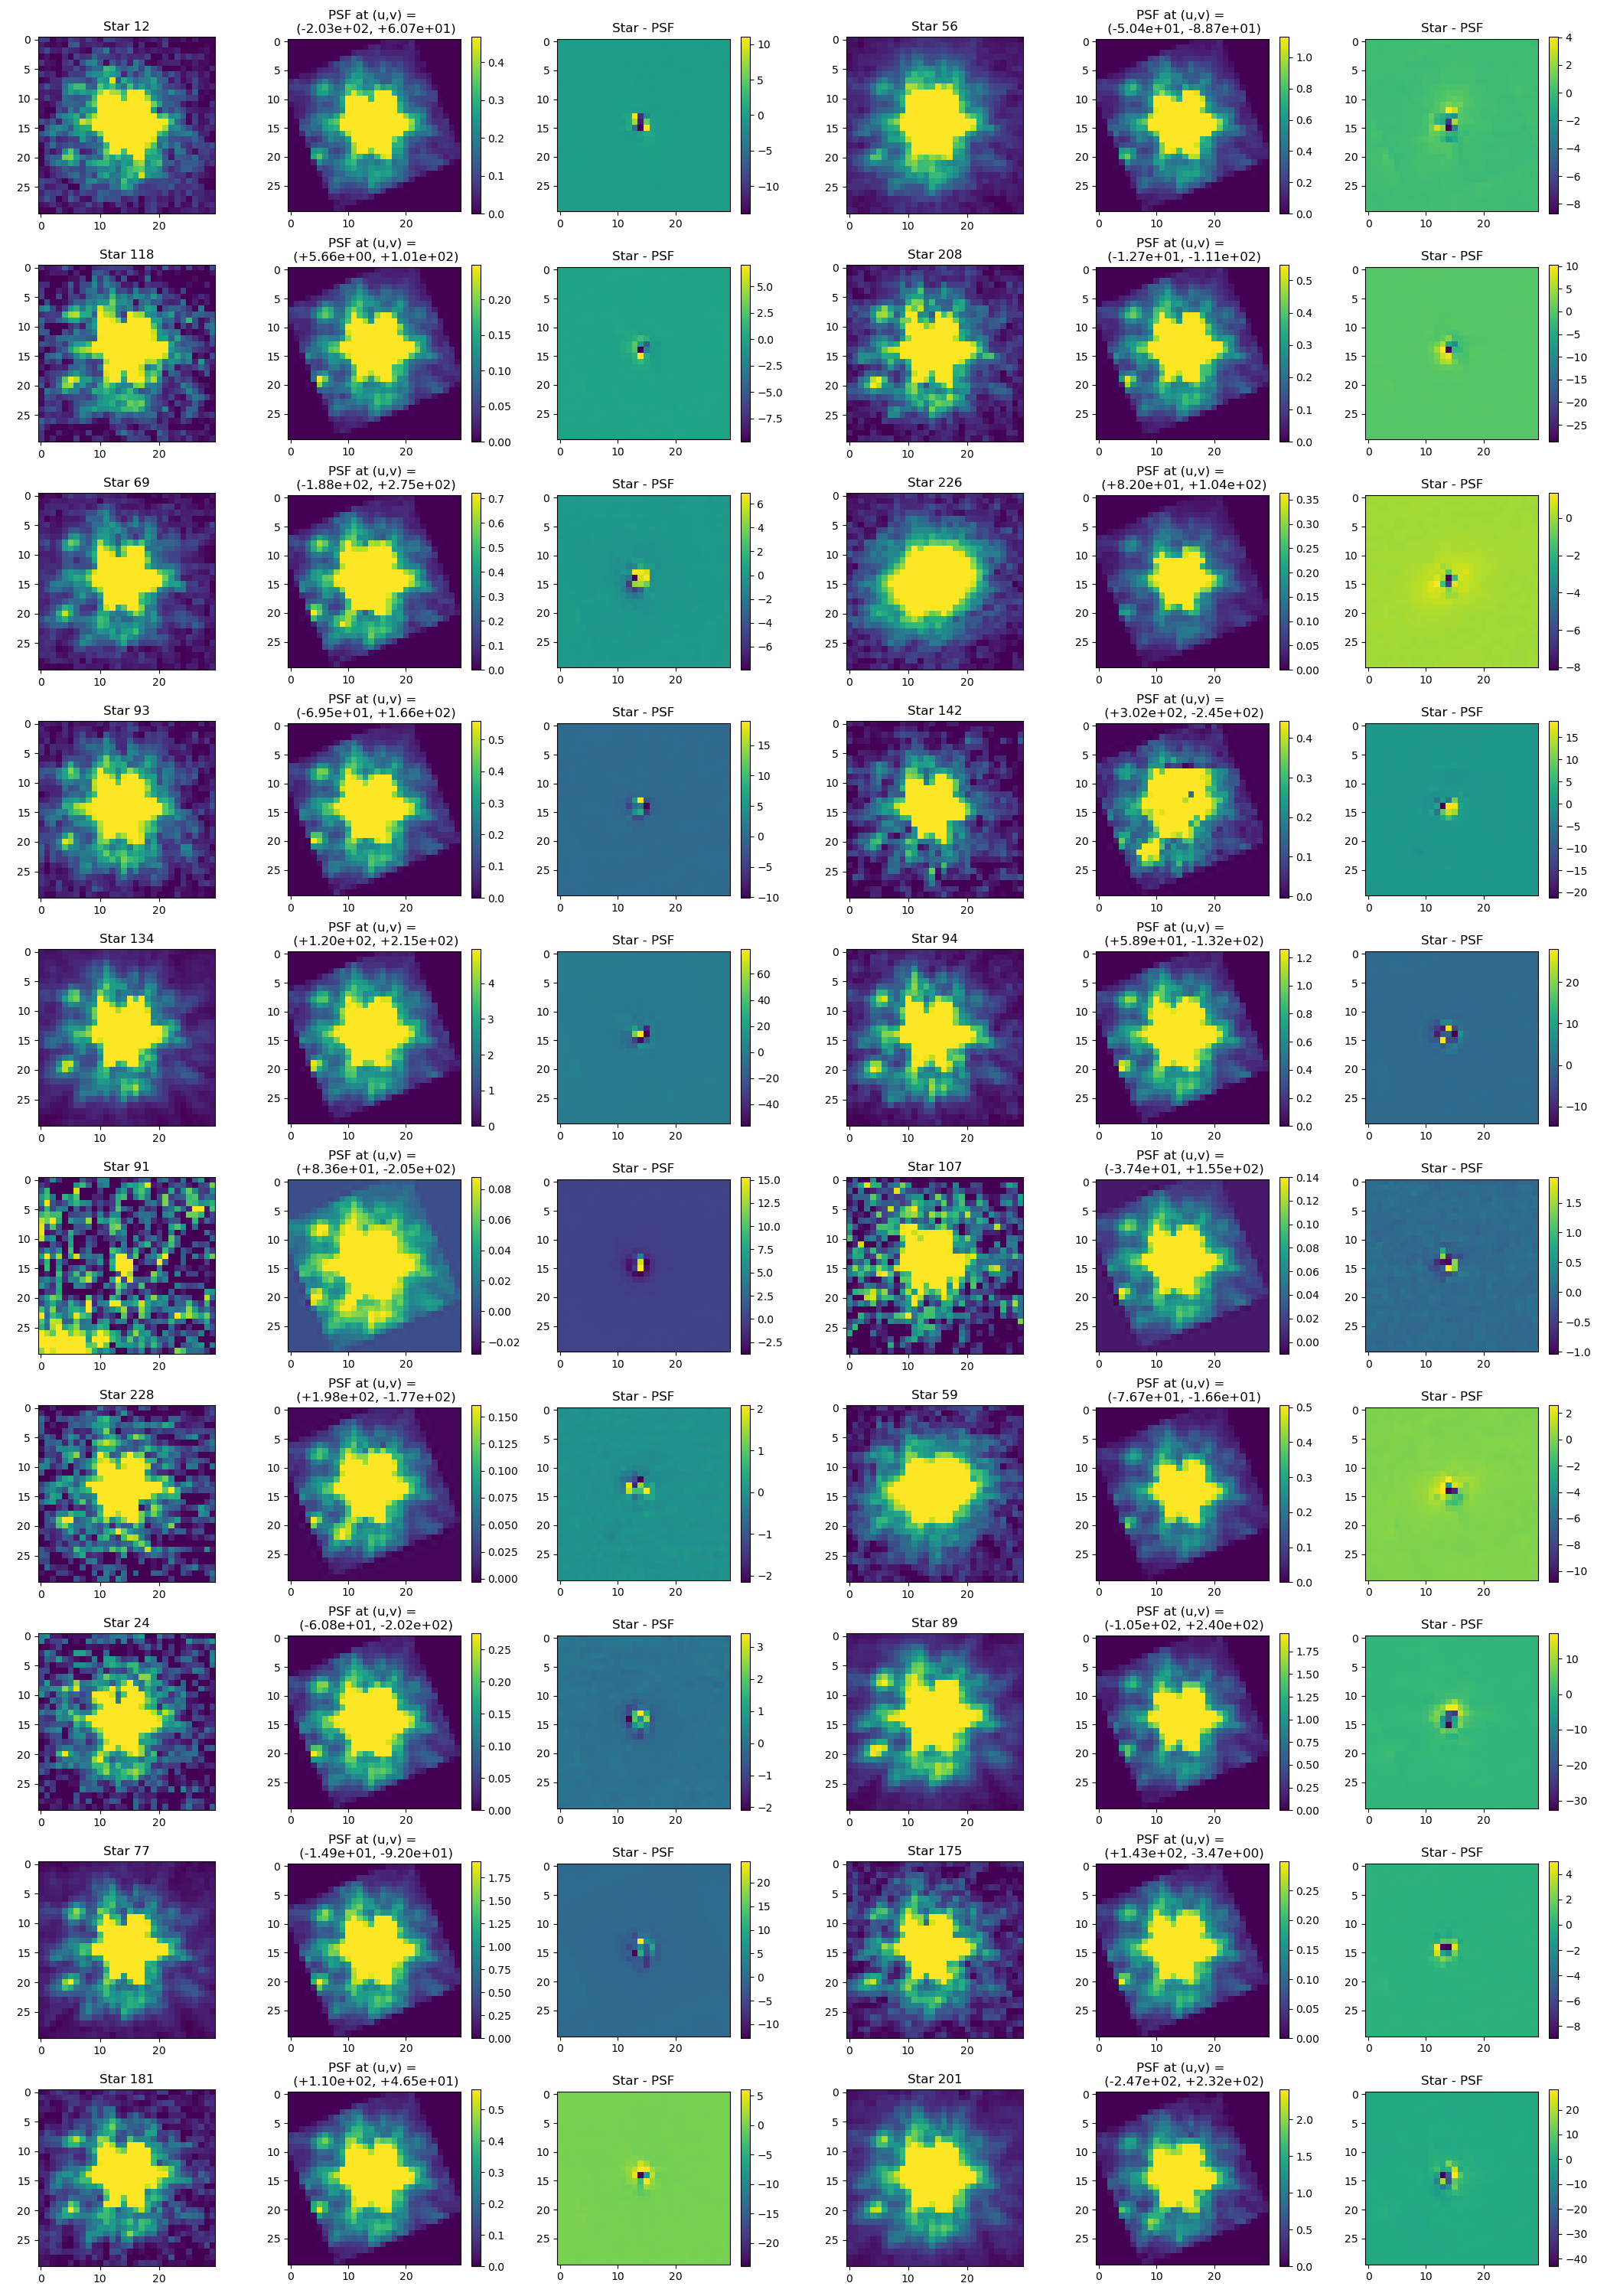
\includegraphics[width=.3\linewidth]{Simulated30mas115/piff_stars.png}
  \end{subfigure}\par\medskip
  \begin{subfigure}{\linewidth}
  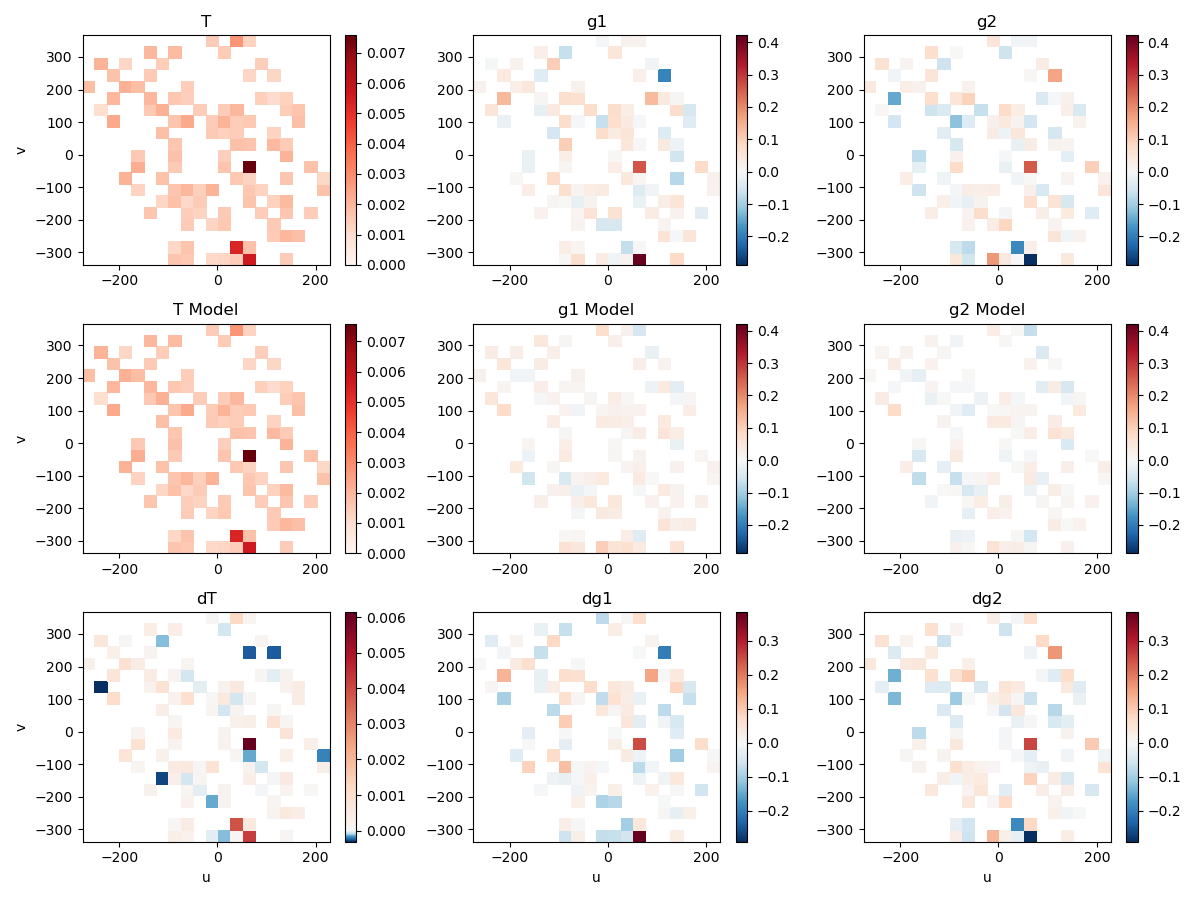
\includegraphics[width=.3\linewidth]{Simulated30mas115/piff_twod.png}\hfill
  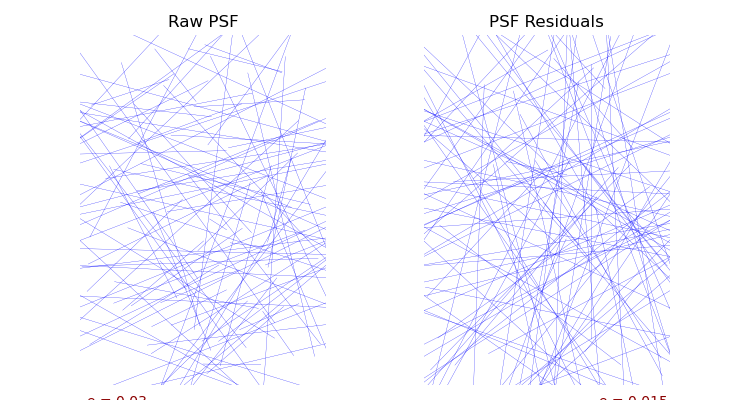
\includegraphics[width=.3\linewidth]{Simulated30mas115/piff_whisker.png}\hfill
  \caption{Simulated30mas115}
  \end{subfigure}\par\medskip


\end{figure}
\begin{figure}[!h]
  \begin{subfigure}{\linewidth}
  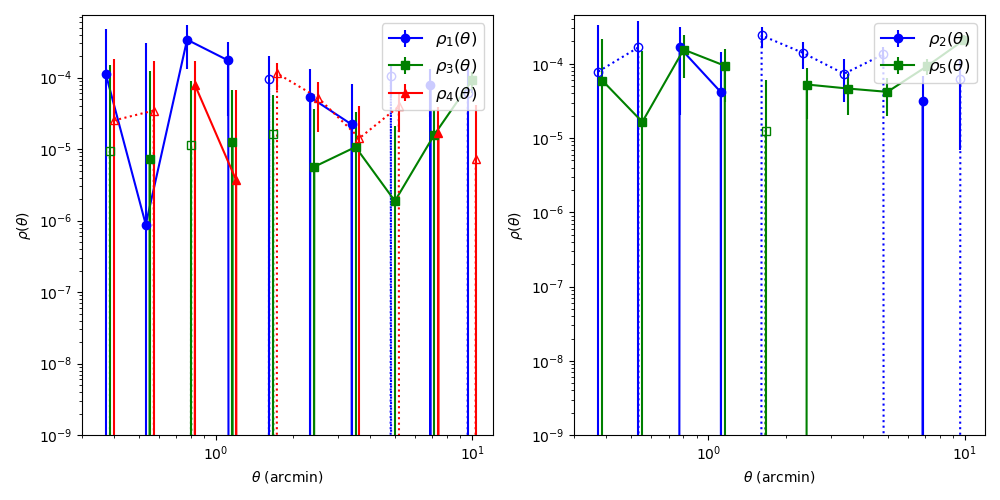
\includegraphics[width=.3\linewidth]{Simulated30mas150/piff_rho.png}\hfill
  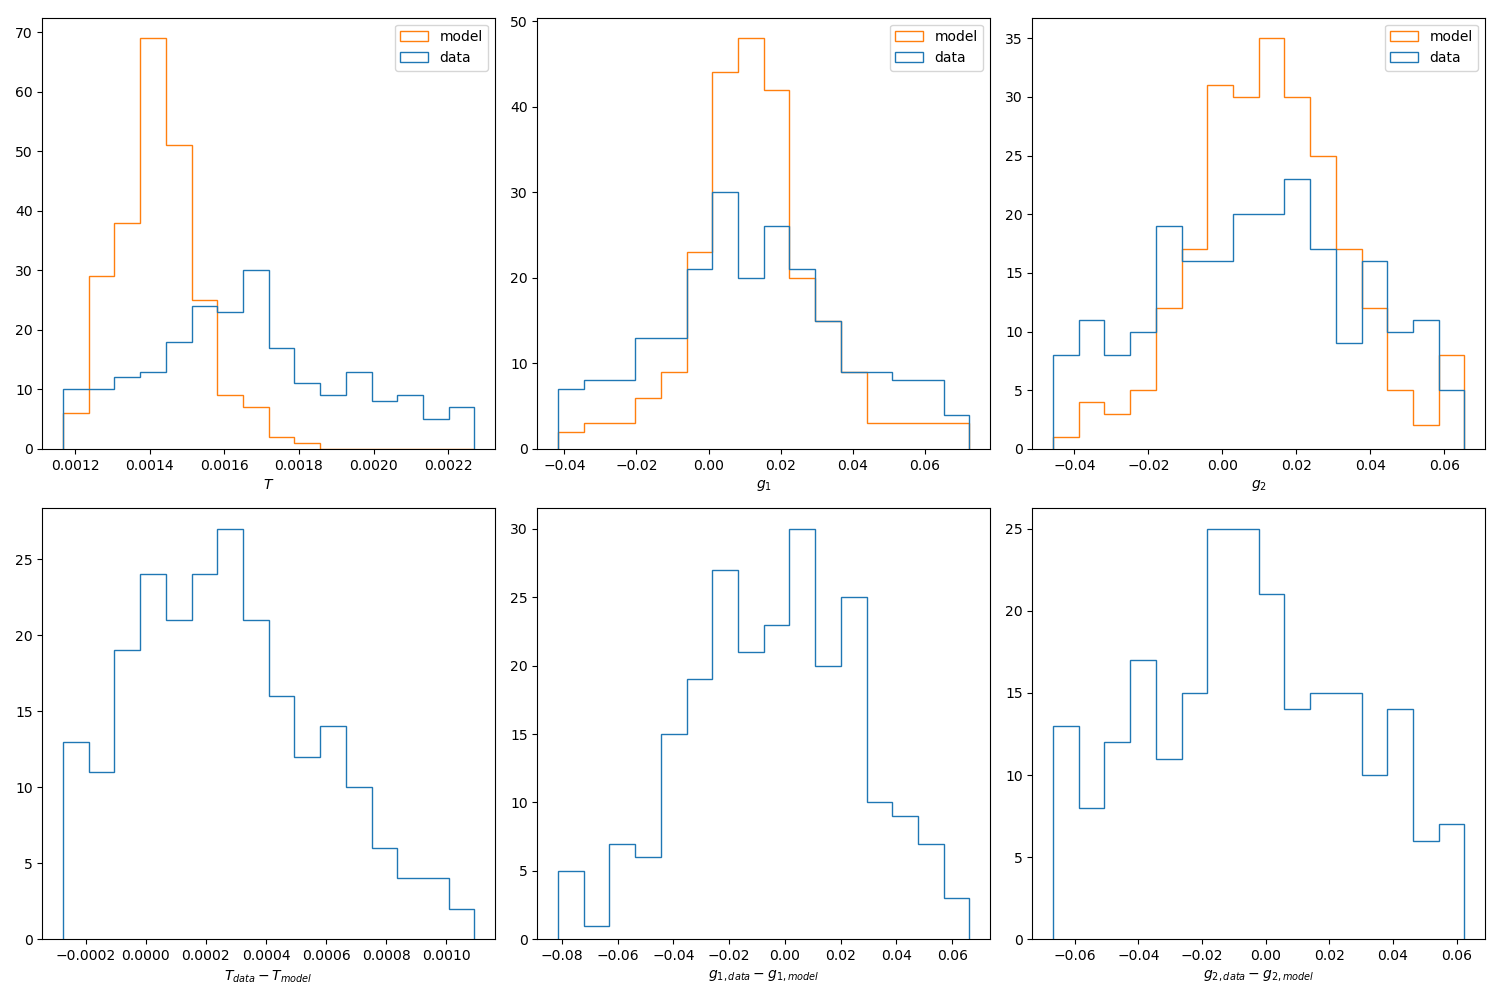
\includegraphics[width=.3\linewidth]{Simulated30mas150/piff_shapes.png}\hfill
  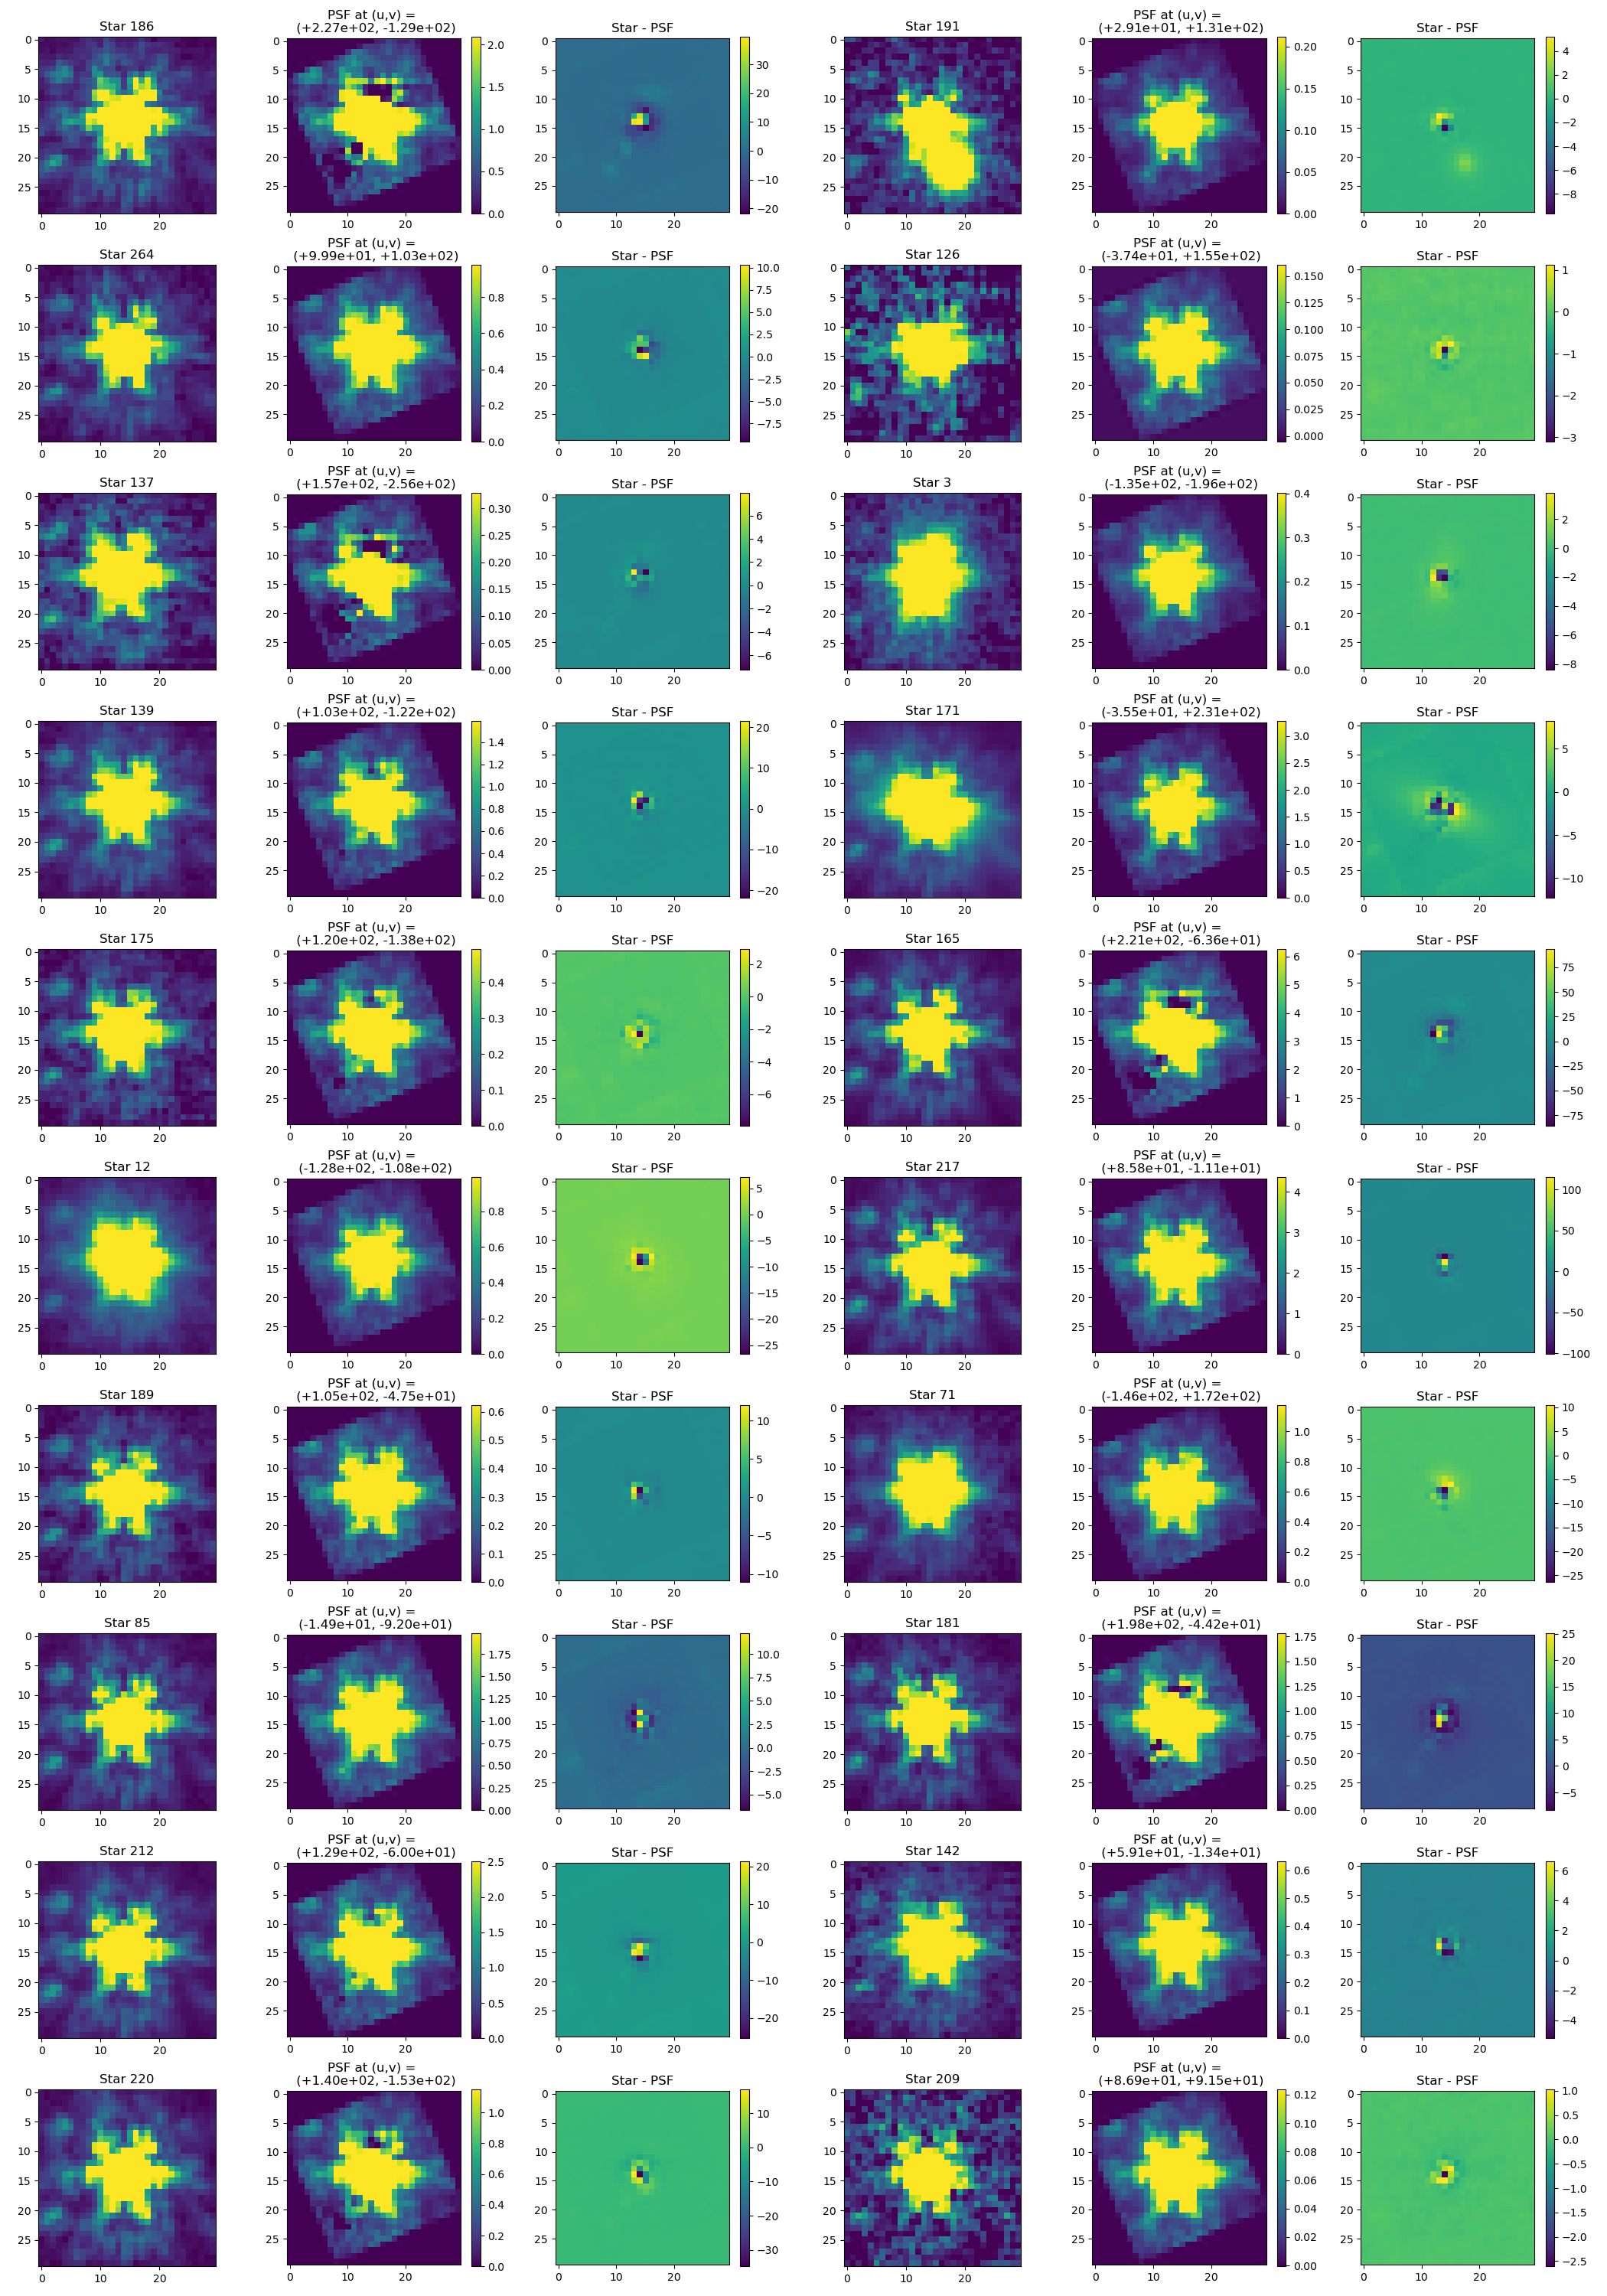
\includegraphics[width=.3\linewidth]{Simulated30mas150/piff_stars.png}
  \end{subfigure}\par\medskip
  \begin{subfigure}{\linewidth}
  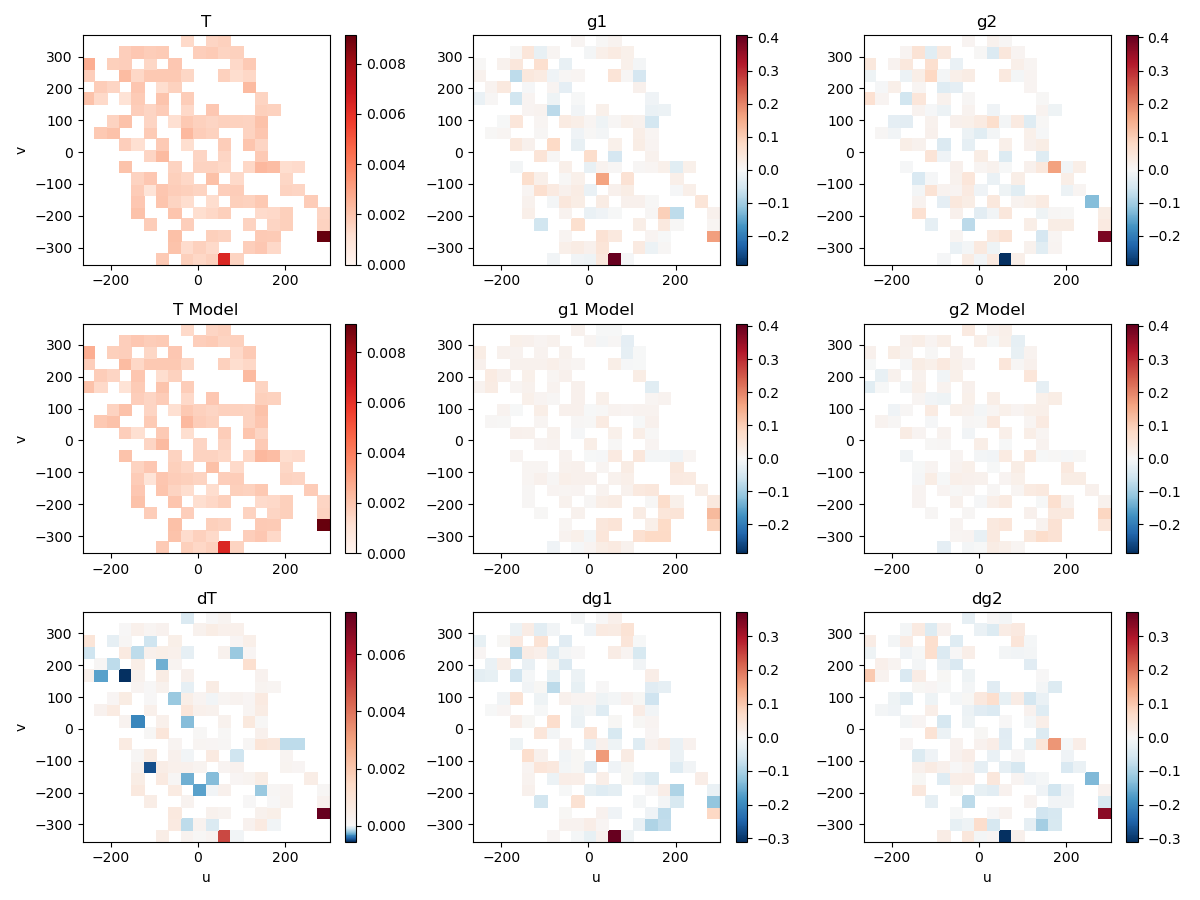
\includegraphics[width=.3\linewidth]{Simulated30mas150/piff_twod.png}\hfill
  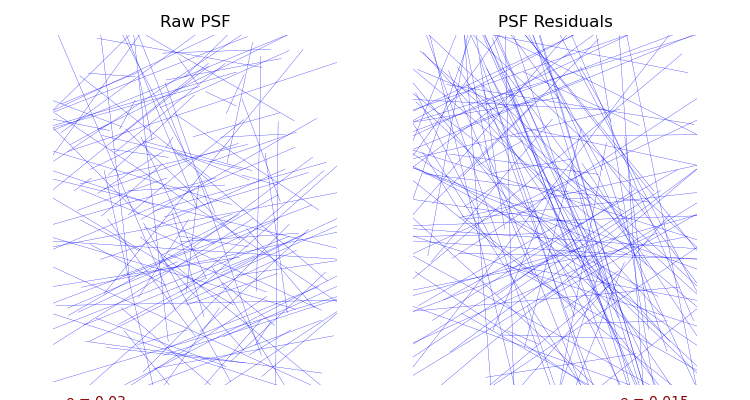
\includegraphics[width=.3\linewidth]{Simulated30mas150/piff_whisker.png}\hfill
  \caption{Simulated30mas150}
  \end{subfigure}\par\medskip


\end{figure}
\clearpage
\clearpage
\noindent {\fbox{\it Another Paper}}\\ 
\begin{itemize}
    \item Full disclosure I have barely read this one, basically just skimmed it, but something I read in the paper you sent me made me think to look for something like this
    \item \href{https://ar5iv.labs.arxiv.org/html/1904.11044}{[Here!]}
\end{itemize}\\
\noindent {\fbox{\it Ascent Award}}\\ 
\begin{itemize}
    \item I think I might apply for one more award to see if I can get paid for part time work during summer 1 $\sim$ 10 hours a week
\end{itemize}
\noindent {\fbox{\it Still to Do}}\\ 
\begin{itemize}
    \item Paper gave me some ideas and confirmed supscisions of a manifold structure to be taken advantage of
    \item Parse through PIFF
    \item Start planning my alternative
    \item Confusion running on real data
\end{itemize}

















\end{document}
%%------------ Arman Shokrollahi--------------%%
